%% TODOS OS CRÉDITOS A:
%%
%% RiSE's latex template for thesis and dissertations
%% http://risetemplate.sourceforge.net
%%
%% (c) 2012 Yguaratã Cerqueira Cavalcanti (yguarata@gmail.com)
%%          Vinicius Cardoso Garcia (vcg@cin.ufpe.br)
%%
%% This document was initially based on UFPEThesis template, from Paulo Gustavo
%% S. Fonseca.
%%

%%% PEQUENAS ADAPTAÇÕES PARA SER USADO NO IFBA:
%%% José Dihego da Silva Oliveira
%%%  jose.dihego@ifba.edu.br

%%
%% INSTRUÇÕES
%%
%%         * Idiom
%%           pt   - Português (default)
%%           en   - Inglês
%%
%%         * Tipos
%%           bsc  - TCC
%%           msc  - MESTRADO
%%           qual - QUALIFICAÇÃO
%%           prop - PROPOSTA
%%           phd  - TESE FINAL
%%
%%         * PAGINAÇÃO
%%           oneside - uma
%%           twoside - duas
%%
%% REFERÊNCIAS
%%          \figref  -- para figura
%%          \tabref  -- para tabela
%%          \eqnref  -- para equação
%%          \chapref -- para capítulo
%%          \secref  -- para seção
%%          \appref  -- para apêndice
%%          \axiref  -- para axioma
%%          \conjref -- para conjectura
%%          \defref  -- para definição
%%          \lemref  -- para lema
%%          \theoref -- para teorema
%%          \corref  -- para corolário
%%          \pgref   -- para página
%%
%%          \citet (from natbib) -- Citação como 
%% parte da narativa
%%          \citep (from natbib) -- Citação
%% entre parêntesis

\documentclass[pt,twoside,onehalfspacing,bsc]{risethesis}

\usepackage{colortbl}
\usepackage{color}
\usepackage[table]{xcolor}
\usepackage{microtype}
\usepackage{bibentry}
\usepackage{subfigure}
\usepackage{multirow}
\usepackage{rotating}
\usepackage{booktabs}
\usepackage{pdfpages}
\usepackage{caption}
\usepackage{lipsum}
\usepackage{sectsty}

\captionsetup[table]{position=top,justification=centering,width=.85\textwidth,labelfont=bf,font=footnotesize}
\captionsetup[lstlisting]{position=top,justification=centering,width=.85\textwidth,labelfont=bf,font=footnotesize}
\captionsetup[figure]{position=bottom,justification=centering,width=.85\textwidth,labelfont=bf,font=footnotesize}

%% Capítlos, seções e sub-seções devem ter o  mesmo tamanho de fonte 12 
\sectionfont{\fontsize{12}{15}\selectfont}
\subsectionfont{\fontsize{12}{15}\selectfont}
\subsubsectionfont{\fontsize{12}{15}\selectfont}
\usepackage{amsmath}
\newcommand{\dd}[1]{\mathrm{d}#1}

%% Atualize com seus dados
\usepackage[linkcolor=black,
            citecolor=black,
            urlcolor=black,
            colorlinks,
            pdfpagelabels,
            pdftitle={Título do meu trabalho},
            pdfauthor={Meu nome},
            breaklinks=true]{hyperref}

\address{FEIRA DE SANTANA}

\universitypt{Instituto Federal de Educação, Ciência e Tecnologia da Bahia }
\universityen{Federal Institute of Bahia
}

\departmentpt{Bacharelado em Sistemas de Informação}
\departmenten{Bachelor in Computer Information Systems}

\programpt{Graduação em Sistemas de Informação}
\programen{Bachelor in Computer Information Systems}

\majorfieldpt{Sistemas de Informação}
\majorfielden{Information Systems}

\title{Seu título compacto, chamativo e esclarecedor}

\date{2019}

\author{Seu nome}
\adviser{Nome orientador}
\coadviser{Nome coorientador}

\def\x{\checkmark}

\begin{document}

\frontmatter

\frontpage

\presentationpage

\begin{fichacatalografica}
	\FakeFichaCatalografica
\end{fichacatalografica}

\banca

\begin{dedicatory}
Dedico este trabalho...
\end{dedicatory}

\acknowledgements
\lipsum[1-4]

\begin{epigraph}[]{Patativa do Assaré}
Sertão, argúem te cantô,
Eu sempre tenho cantado
E ainda cantando tô,
Pruquê, meu torrão amado,
Munto te prezo, te quero
E vejo qui os teus mistéro
Ninguém sabe decifrá.
A tua beleza é tanta,
Qui o poeta canta, canta,
E inda fica o qui cantá.
\end{epigraph}

\resumo
% Escreva seu resumo em português no arquivo resumo.tex
{\parindent0pt
	\vspace*{-.5cm}

Na medida em que os sistemas computacionais se tornam mais pervasivos, a demanda por métodos de desenvolvimento rigorosos e composicionais cresce dramaticamente. No desenvolvimento baseado em componentes (CB-MDD), sistemas complexos (muitas vezes humanamente intangíveis) são construídos a partir de elementos mais simples, chamados componentes. Para atingir os objetivos desta abordagem na direção de torná-la uma disciplina formal de desenvolvimento, componentes e regras de composição devem ser formalizados. Além disso, considerando que os requisitos de um sistema estão em constante evolução, necessitamos de mecanismos para refinar e estender de forma confiável tais sistemas. O modelo de componentes BRIC formaliza os conceitos chave da abordagem CB-MDD, além de garantir corretude por construção se baseando em regras de composição que preservam propriedades comportamentais. BRIC, porém, por não possuir relações de extensão, não suporta evolução de modelos baseados em componentes.

Neste trabalho propomos relações de herança e refinamento para BRIC. Definimos uma semântica congruente que considera tanto a estrutura quanto o comportamento de componentes. Definimos refinamento como uma relação de pré-ordem, a qual é monotônica em relação as regras de composição de BRIC. Estendemos este modelo de componentes com suporte a extensibilidade via herança. As relações propostas permitem extensão de funcionalidade, ao mesmo tempo em que preservam conformidade de serviços, a qual é definida em termos de uma noção de convergência. Estabelecemos também uma conexão algébrica entre extensibilidade de componentes e refinamento. Até onde estamos cientes, este trabalho é pioneiro no desenvolvimento de noções de herança de componentes para uma abordagem CB-MDD formal e consistente. 

Também integramos o paradigma orientado a aspectos em BRIC. Contribuímos com uma abordagem para capturar, especificar e adotar aspectos no desenvolvimento confiável de sistemas baseados em componentes. Estabelecemos que componentes estendidos por aspectos preservam convergência, o que garante conformidade de serviços. Além disso, desenvolvemos uma conexão entre herança e aspectos, apresentando herança como um mecanismo para definir famílias de componentes e aspectos para capturar conceitos ortogonais sobre as mesmas.

Ilustramos a relevância prática das relações propostas através de três estudos de caso. No primeiro, modelamos um sistema autônomo de cuidados médicos, estendido pela adição de novas funcionalidades via herança e pela modularização de conceitos transversais de forma reusável e manutenível via aspectos. Na sequência, modelamos um sistema bancário, cujas funcionalidades são progressivamente implementadas e estendidas pelo uso de herança e refinamento. Finalmente, modelamos um sistema P2P cujo tráfico é reduzido por extensão via herança.

\begin{keywords}
herança de componentes. refinamento de componentes. correção por construção. \textit{design} orientado a aspectos para modelos de componentes. convergência comportamental. CSP
\end{keywords}

}

\abstract
% Escreva seu resumo em inglês no arquivo abstract.tex
{\parindent0pt
	
As computer systems become ubiquitous, the demand for rigorous and compositional development methods increase dramatically. In the component-based model driven development (CB-MDD) approach, complex systems (sometimes intractable by humans) are build from simple elements, called components. To achieve the CB-MDD goals towards becoming a rigorously development discipline, components and composition rules must be formalised. Moreover, as requirements continuously evolve, there must be mechanisms to refine and safely extend component-based systems. The BRIC component model formalises the CB-MDD core concepts and supports a constructive design based on composition rules that preserves behavioural properties, but do not provide support for component model evolution. 

In this work we propose inheritance and refinement relations for BRIC. We define a congruent semantics for this model that considers component structure and behaviour. We define refinement as a preorder relation, which is monotonic with respect to the BRIC composition rules. We enhance this component model with support for extensibility via inheritance. The proposed relations allow extension of functionality, whilst preserving service conformance, which we define by means of a convergence notion. We also establish an algebraic connection between component extensibility and refinement. As far as we are aware this is the first time component inheritance relations are developed for a formal and sound CB-MDD approach.

We also integrate the aspect-oriented paradigm into BRIC. We contribute with an approach to capture, specify and use aspects to safely evolve component-based systems. We establish that components extended by aspects preserve the proposed convergence relation that guarantees service conformance. Furthermore, we establish a connection between component inheritance and aspects, presenting inheritance as a mechanism to define families of components and aspects to capture orthogonal concerns over them.

The practical relevance of the proposed relations is illustrated by three case studies. One is an autonomous healthcare system, which evolve by the addition of new functionalities via inheritance and by the modularisation of its crosscutting concerns in a reusable and maintainable manner with aspects. Another case study is a bank system, whose functionalities are progressively realised and extended by refinement and inheritance, respectively. Finally, we model a P2P system extended by inheritance to reduce the network traffic.

\begin{keywords}
component inheritance. component refinement. correctness by construction. component-based aspect-oriented design. behavioural convergence. CSP
\end{keywords}

}

% List of figures
\listoffigures

% List of tables
\listoftables

% List of acronyms
% Acronyms manual: http://linorg.usp.br/CTAN/macros/latex/contrib/acronym/acronym.pdf
\listofacronyms
\begin{acronym}[ACRÔNIMOS] 
\acro{lts}[LTS]{labelled transition system}
\acro{serpro}[SERPRO]{Serviço Federal de Processamento de Dados}
\end{acronym}

% Summary (tables of contents)
\tableofcontents

\mainmatter

\chapter{Introdução}
\label{cap:introducao}

O desenvolvimento tradicional de software tem se mostrado incapaz de lidar de modo eficiente com a evolução constante que os artefatos de software estão sujeitos durante seu ciclo de vida \citep{Kleppe:2003}. Os artefatos produzidos nas fases iniciais de desenvolvimento, como documento de requisitos e digramas UML, tem seu conteúdo cada vez mais distanciado do estado atual do software à medida que avançam as etapas de codificação e testes. Durante a etapa de manutenções, essa distância torna sem valor os documentos textuais e diagramas inicialmente produzidos.
A manutenção sem documentação acaba sendo feita totalmente via inspeção de código, o que torna o processo bastante improdutivo. Da mesma forma, a atualização constante dos documentos e diagramas torna o processo de desenvolvimento menos produtivo \citep{Kleppe:2003}. Além dos problemas com manutenção e produtividade, existem graves problemas acerca da interoperabilidade e dependência de plataforma, dado à vasta gama de novas tecnologias e plataformas de software que surgem cada vez mais rapidamente.
A abordagem de desenvolvimento orientada a modelos é uma resposta da academia a essa série de problemas que se apresenta ao mercado como uma alternativa ao desenvolvimento tradicional e seus artefatos \citep{Frankel:2002}. MDA (Model Driven Architecture) é um framework de desenvolvimento de software, definido pela OMG (Object Management Group), que propõe a modelagem como atividade central na construção de software.
 	A atividade de modelagem começa com a elaboração de um modelo independente de computação (CIM), que após a fase de análise origina um modelo independente de plataforma (PIM). A fase de projeto, levando em consideração a tecnologia de implementação, utiliza o PIM para gerar um modelo específico de plataforma (PSM) que nas fases seguintes é transformado em código. A cada fase os modelos se tronam menos abstratos e mais relacionados com a tecnologia adotada. 
	A definição de MDA prevê que transformações entre os níveis de modelos, ou mesmo reestruturações em um dado nível, ocorram de forma automática preservando sempre a conformidade entre os vários modelos. Nessa abordagem, desenvolvedores focariam seus esforços na criação de modelos PIM que melhor suportassem as regras de negócio do sistema e através do uso de ferramentas de transformação seriam gerados, na seqüência, modelos PSM e código fonte.
	Todo o esforço dos desenvolvedores concentrado na definição de um modelo PIM, gera ganho de produtividade e qualidade no sistema final, já que a complexidade da geração do PSM (e código fonte) torna-se responsabilidade das ferramentas de transformação. Um único PIM pode gerar PSMs para diferentes plataformas, aumentando assim a portabilidade do sistema. A manutenção, nessa abordagem, também é bastante favorecida, pois o PIM assume o papel de documentação de alto-nível do sistema e está sempre de acordo com o estado atual do mesmo, favorecendo a incorporação de novos requisitos através de mudanças no PIM seguidas de gerações automáticas de PSM e código \citep{Frankel:2002}.
	Um tipo de transformação, previsto no framework MDA, é destinado a reestruturar o modelo mantendo-o no mesmo nível. Reestruturação (refactoring) é definida em como sendo uma transformação de uma abstração em outra, de mesmo nível, preservando o comportamento externo do sistema (funcionalmente e semanticamente). A aplicação de refactorings tem como objetivo aumentar a qualidade do software através da inserção ou melhoria de requisitos não funcionais ou soft-goals (como, por exemplo, modularidade, manutenabilidade, reusabilidade). A pouca disponibilidade de ferramentas que automatizem as transformações, peça central do framework MDA, é um entrave a sua utilização plena no mercado \citep{Frankel:2002}. 


\begin{figure}[htp]
\centering
  \caption[]{\ac{lts} Estados, transições e eventos}
  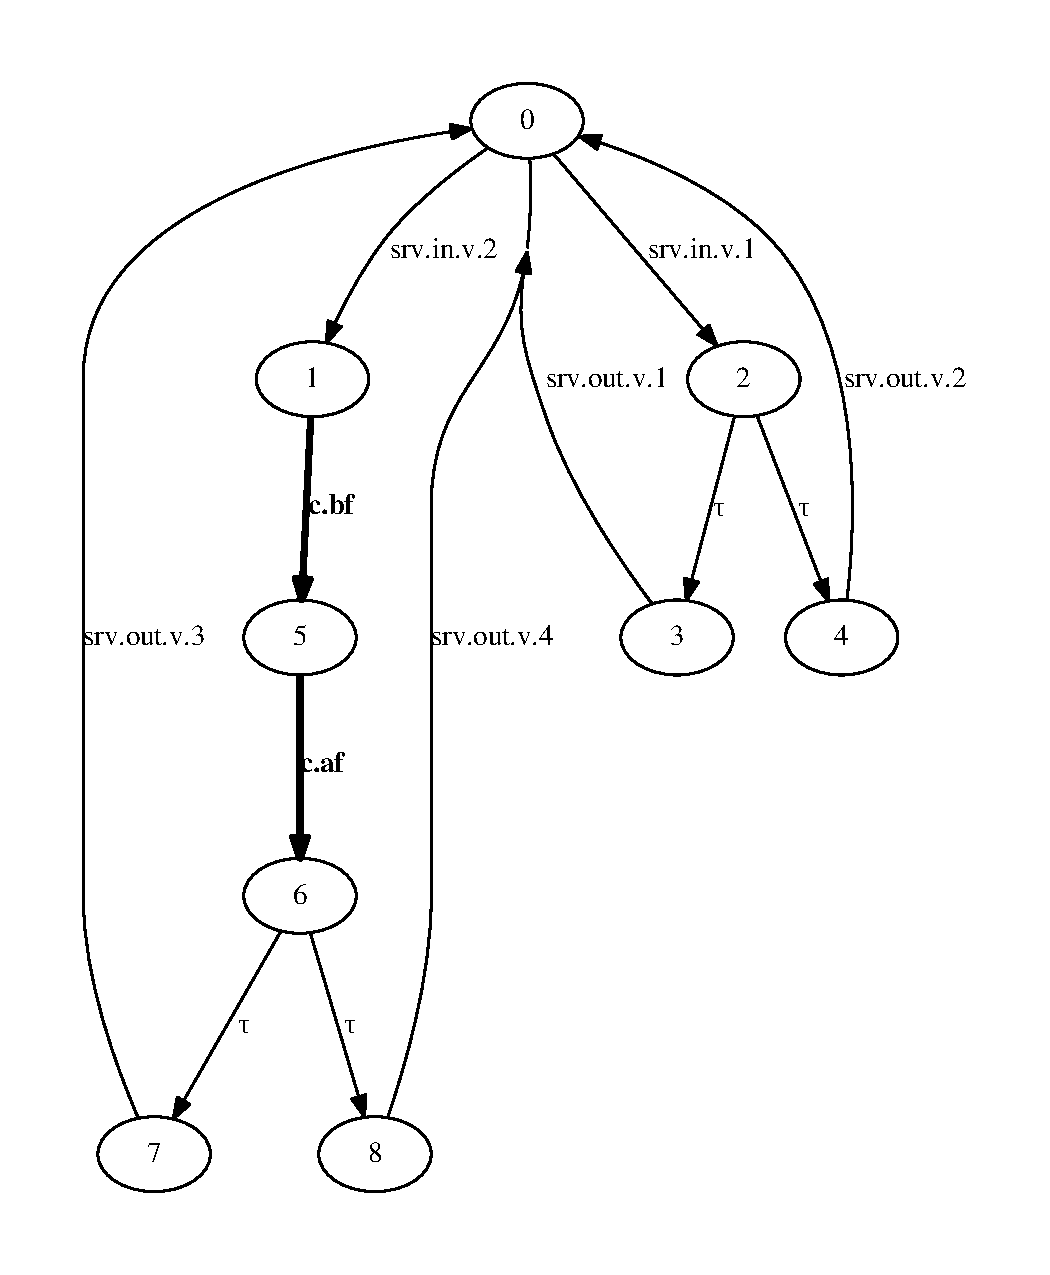
\includegraphics[width=\columnwidth]{imagens/P1andSRV-eps-converted-to.pdf}
  \footnotesize{Fonte: próprio autor}
  \label{fig:minha-imagem1}
\end{figure}

Isso é demostrado na \figref{fig:minha-imagem1}, onde...

Observe a \tabref{tbl:historico_revisoes}, é possível ver...

A equação matemática...

\begin{equation}
Z=\min E \int_{0}^{\infty} \exp(-\rho t)\left\{ \alpha^2[r(t)-x(t)]^2+
  \left[\lambda ^ {-1}\frac{\dd{x(t)}}{\dd{t}}\right]^2 \right\} \dd{t}
\end{equation}

 \section{Suporte}
Para terminar seu TCC é preciso:

\begin{enumerate}
  \item Estudar.
  \item Estudar mais.
  \item Dormir para estudar
  \item Estudar
  \item Voltar ao passo 1.
\end{enumerate}

\section{Proposta}
\lipsum[2-2]



\section{Organização deste trabalho}

\lipsum[2-2]

\chapter{Fundamentos}

\section{Introdução}

\lipsum[1-4]

\section{Seção}

\lipsum[2-4]

\subsection{Subseção}

\lipsum[2-4]
\include{capitulos/desenvimento}
\chapter{Conclusão}

\section{Introdução}

\lipsum[1-4]

\section{Seção}

\lipsum[2-4]

\subsection{Subseção}

\lipsum[2-4]

% References

\begin{references}
  \bibliography{referencias}
\end{references}

% Appendix

\theappendix
\chapter{Tabelas}
\label{ap:apendice}

\begin{table}[htp]
	\caption{Histórico de Revisões}
	\label{tbl:historico_revisoes}
	\centering
	\rowcolors{2}{lightgray!30}{white}
	 \centering
    \begin{tabular}[pos]{|m{2cm} | m{7.2cm} | m{3.8cm}|} 
      \hline
      \cellcolor[gray]{0.9}
      \textbf{Date} & \cellcolor[gray]{0.9}\textbf{Descrição} & \cellcolor[gray]{0.9}\textbf{Autor(s)}\\ \hline
      \hline
      \small xx/xx/xxxx & \small <Descrição> & \small <Autor(es)> \\ \hline      
      \small xx/xx/xxxx &
      \begin{small}
        \begin{itemize}
          \item Exemplo de;
          \item Revisões em lista;
        \end{itemize}
      \end{small} & \small <Autor(es)> \\ \hline 
    \end{tabular}
\end{table}


\end{document}
